\definecolor{ackblue}{HTML}{365f91}
\titleformat{\chapter}[display]
  {\normalfont\bfseries\color{ackblue}\filcenter}
  {\Large\MakeUppercase{Chapter \thechapter}}{0pt}
  {\Large\MakeUppercase}
\titleformat{\section}
  {\color{ackblue}\bfseries}
  {\thesection.}{0.5em}{}
\titleformat{\subsection}
  {\color{ackblue}\bfseries}
  {\thesubsection.}{0.5em}{}

\chapter{INTRODUCTION}

\section{Background}

Mesh data from scanners or photogrammetry is rarely watertight. Self-occlusion, low-confidence regions, glossy surfaces, and post-process editing all introduce holes. The presence of a hole is enough to break rendering (the back side becomes visible through it), most physical simulations (which assume a closed domain), and 3D-print slicers.

Standard hole fillers, such as ear clipping or the advancing-front method behind MeshLab's \texttt{Close Holes}, close the topological gap but produce a patch that is essentially flat. On a sphere this is immediately visible as a dimple. More sophisticated alternatives exist --- Poisson reconstruction, thin-plate splines --- but they either reshape the entire mesh or require solving a fourth-order PDE, neither of which fits an interactive plugin model.

The hole-filling problem appeared on the Advanced Computer Graphics project list, but only the problem itself was specified, not the approach. NFD was chosen after a short literature survey: the Verdera et al.\ paper on inpainting surface holes offered the most direct route from boundary normals to a curved patch, and most of its machinery (cotangent Laplacian, heat equation, sparse linear solvers) was already covered in the course.

\begin{figure}[H]
    \centering
    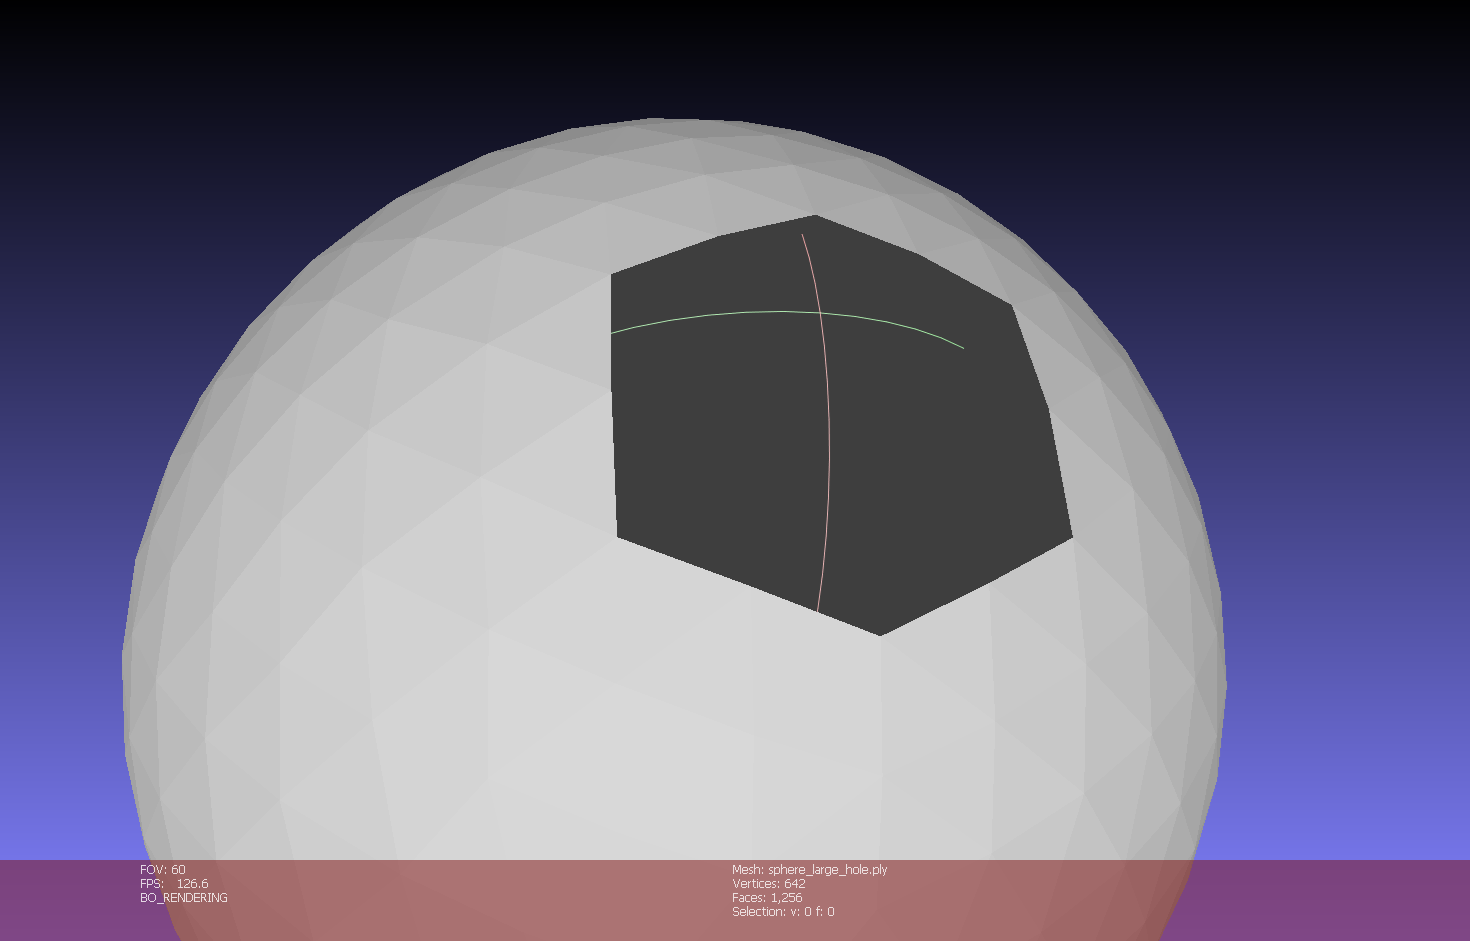
\includegraphics[width=0.45\textwidth]{figures/fig_teaser_hole.png}
    \hfill
    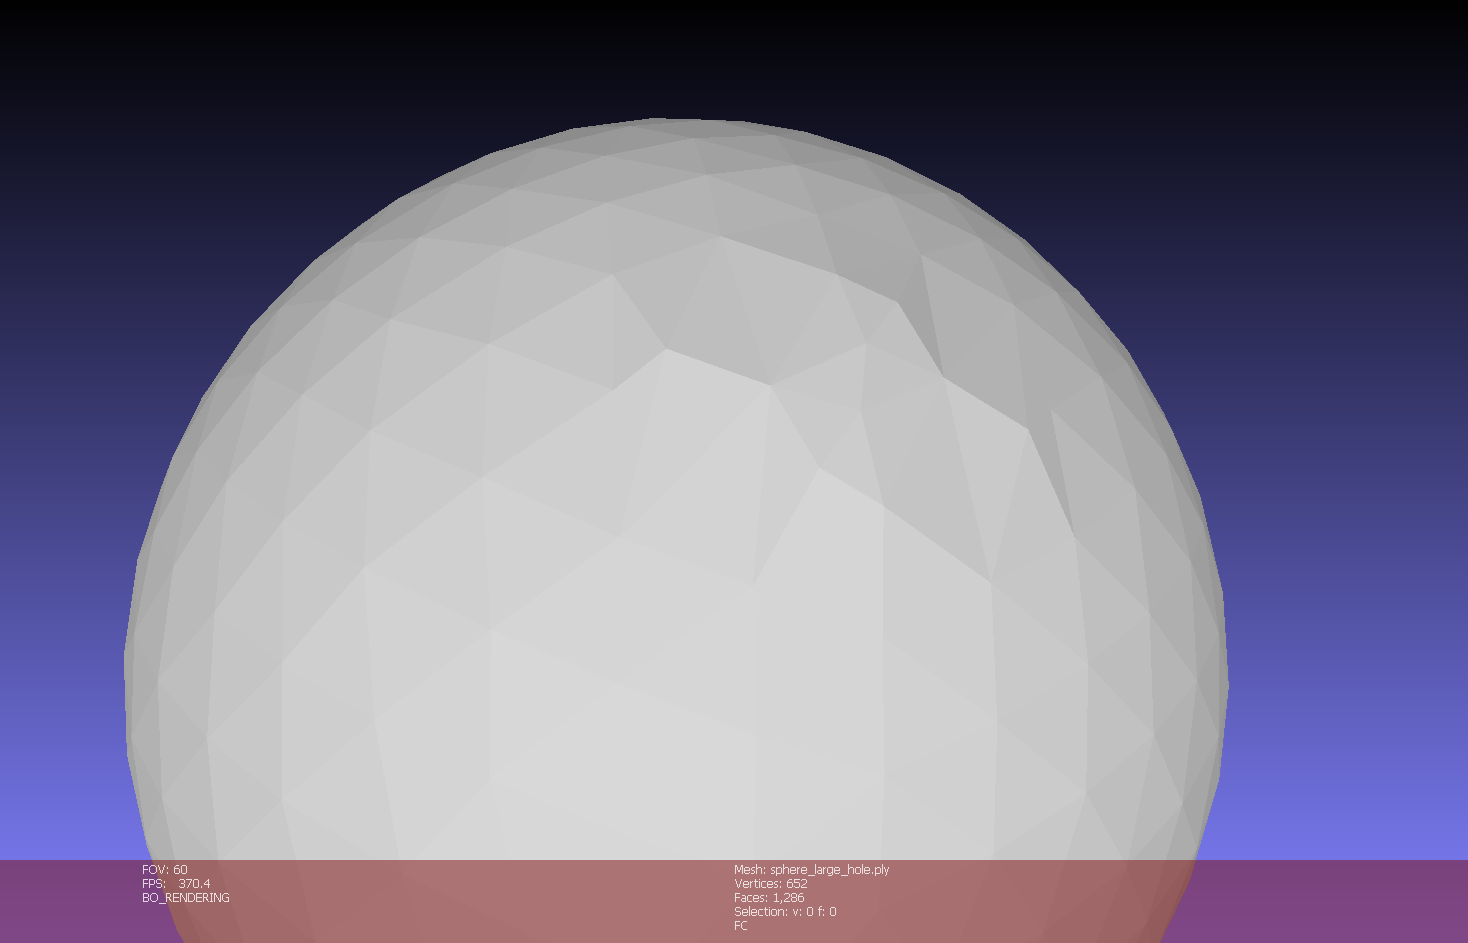
\includegraphics[width=0.45\textwidth]{figures/fig_teaser_filled.png}
    \caption{Input mesh with a hole (left) and the NFD result (right).}
    \label{fig:teaser}
\end{figure}

Normal Field Diffusion (NFD) sits between these extremes. It triangulates the hole as a flat patch first, then diffuses the boundary normals across the patch interior using a discrete heat equation, and finally displaces each interior vertex along its diffused normal by an amount estimated from the boundary geometry. The patch ends up curved, matches the surrounding surface, and the rest of the mesh is left alone.

\section{Problem and scope}

Given a mesh $\mathcal{M} = (V, F)$ with one or more boundary loops, the goal is to add vertices and faces so that each loop becomes interior, the patch joins the surrounding surface continuously, and the new triangles are roughly the same size and shape as their neighbours. The topological closure is trivial. Triangle quality is handled by standard heuristics. The hard part is geometric continuity, which is what this report focuses on.

The implementation is a self-contained MeshLab plugin in C++ on top of VCGlib and Eigen. It processes one hole at a time, leaves everything else untouched, and exposes seven parameters in the standard filter dialog. Evaluation uses MeshLab's built-in Hausdorff sampler against ground-truth meshes generated from the same source models.

\section{Outline}

Chapter~2 surveys related work and places NFD in context. Chapter~3 collects the mathematical background --- discrete Laplace--Beltrami, the heat equation, implicit Euler, Taubin smoothing. Chapter~4 walks through the seven pipeline stages. Chapter~5 covers the plugin implementation. Chapter~6 reports the Hausdorff measurements and compares NFD with MeshLab's \texttt{Close Holes} filter. Chapters~7 and~8 discuss limitations and conclude.
